\Chapter{Neurális hálók}

A neurális hálózattokat gyakran hasonlítjuk az emberi agy működéséhez. Ha körültekintően szemügyre vesszük agyunk működését, akkor azt tapasztaljuk, hogy neuronokból és közöttük felépülő kapcsolatokból áll össze. A külvilágból érkezett ingereket értelmezhetjük úgy, mint egy bemenetet, amit az agyunkban lévő neuronok feldolgoznak. 

\begin{center}
	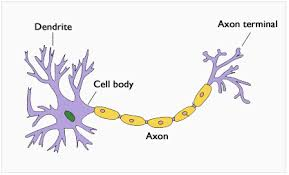
\includegraphics[scale=1.0]{images/neuron.png}
\end{center}

A kutatók az agy felépítését vizsgálva egy olyan matematikai modellt dolgoztak ki, amely   reprezentálni próbálja az agyban található neuronokat és a közöttük lévő kapcsolatokat. Ezt a modellt nevezzük neurális hálónak vagy neurális hálózatnak.  

A neurális hálózatot alkotó neuronok úgynevezett rétegekbe rendeződnek. Háromféle réteget különbözetünk meg, a \textbf{\textit{bemeneti}}, a \textbf{\textit{kimeneti}} és a \textbf{\textit{rejtett réteget}}. Bemeneti és kimeneti rétegből minden hálózatban egy darab van, rejtett rétegből azonban tetszőleges számú lehet. 

A hálózatban a rétegeket élek kötik össze egymással, amelyekhez egyenként egy-egy \textbf{\textit{súly}} tartozik. A neuronok a bemeneti éleiken kapott értékek és a súlyok segítségével bizonyos műveleteket végeznek el, majd az eredmény a kimeneti éleiken keresztül továbbítják a következő réteg neuronjai felé. 

A tanítási folyamat elvégzésekor a hálózatba olyan bemenetet juttatunk, amelyhez tartozó kimenet ismert. A bemenetet végig futtatjuk a hálózat rétegein, majd a kimeneti réteg által szolgáltatott eredményt összehasonlítjuk a kimenet várt értékével. A két érték közötti eltérést a hálózat \textit{\textbf{hibájának}} nevezzük. A tanítás folyamán a hálózat súlyait úgy változtatjuk, hogy ez a hiba lehetőleg minél kisebb legyen. A hálózat betanítása után már olyan bemeneteket is megadhatunk, amelyeknek már nem ismerjük a kimenetét, és a hálózat ezekre is képes hibahatáron belüli kimenetet produkálni.\\

\begin{figure}
	\centering
	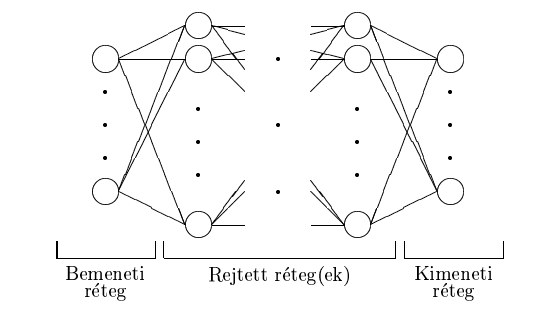
\includegraphics[scale=0.75]{images/ANNLayers.png}
	\caption{Egy általános felépítésű neurális hálózat}
\end{figure}

\begin{Large}
Perceptron
\end{Large}

Az egyszerűség kedvéért vizsgáljunk meg egy olyan neurális hálózatot, amelynek egyetlen neuronnal rendelkezik. Ezt szokás \textbf{\textit{Perceptron}}-nak is nevezni. 

Részei: 

\textbf{\textit{Bemenet}}: Az kiértékelendő adat (ember számára ingerek), amit általában egy vektor (\(x\)) reprezentál. 

\textit{\textbf{Súlyok}}: Két neuron közötti kapcsolat. Egy valós szám (eleinte véletlenszerűek). A hálózat súlyait (W) mátrixba tároljuk el.  

\textbf{\textit{Összegző csomópont}}: A bemeneteket összeszorozza a megfelelő súlyokkal és ezek összegét képezi. Tulajdonképpen mátrix szorzásról van szó.  

\[v(n) = \sum_i^{n}(w_ix_i)\]

\textit{\textbf{Aktivációs függvény}}: Egy olyan függvény ($\varphi$), ami leképezi a kapott összeget egy kisebb intervallumba pl. [0,1] vagy [-1,1] között. 

\textbf{\textit{Kimenet}}: A leképezett értékünk lesz a kimenetünk (\(y\)). 

\begin{center}
	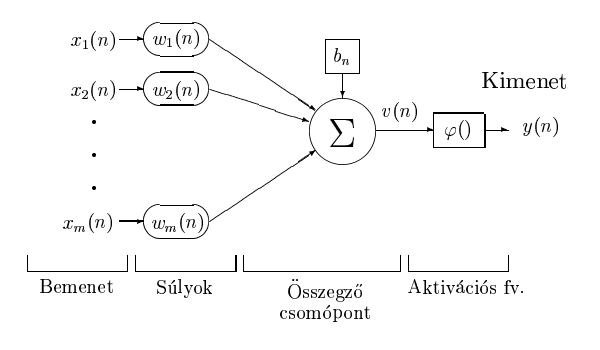
\includegraphics[scale=0.6]{images/ANNParts.png}
\end{center}

\marginnote{\textit{Mi lenne ha az összes generált súly 0 értékű?}}[-0.66cm]

A képen láthatunk egy \(b_n\) változot másnéven bias, amit most nem részleteznék. Alapvetően arra való hogy aktiváljon egy neuront. A \(b(n)\)-hez tartozó súly (\(w_b\)) általában -1 vagy 1.\\


{\Large Backpropagation}

Amennyiben az \(x(n)\) bemenethez tartozó ideális kimenetet \(d(n)\)-nel jelöljük, illetve \(y(n)\) jelenti a hálózat által az \(x(n)\) bemenetre adott kimenetét, a neurális hálózat négyzetes hibáját a következőképpen értelmezzük: 

\[ \varepsilon = (d(n) - y(n))^2\]

Ezt a hibát akarjuk a tanítási eljárás során minimálisra csökkenteni. Természetesen az lenne az ideális, ha a hibát egészen nullára tudnánk redukálni, de ez általában nem sikerül, ezért meg kell elégednünk egy kellően kicsiny hibaküszöbbel. 